\chapter{Спектральный метод генерации синтетической турбулентности} \label{chapt2}

На сегодняшний момент существует достаточно много методов задания турбулентных флуктуаций на входных границах или на границах раздела между двумя подобластями вычислительной области с различными моделями. Их можно подразделить, например, по необходимости в сторонних сопутствующих моделирования, по способу генерации и так далее. Например, в ~\cite{shur2014synthetic} методы генерации разделяют на 5 групп: методы использующие сторонние вычислительные эксперименты, методы переноса турбулентности, методы генерации «синтетической» турбулентности, метод введения объемных источников, метод введения генератора вихрей. Методы относящиеся к каждой из этих групп имеют различные недостатки и достоинства, некоторые из которых будут описаны далее. В первую очередь необходимо обратить внимание на такие аспекты как: область адаптации – то есть область, необходимая для перехода от сгенерированного турбулентного поля к полю, удовлетворяющему уравнениям движения, число вводимых (используемых) параметров. Так же необходимо уделить внимание к программному «дизайну»; вычислительная сложность алгоритма, требуемая память, возможность к распараллеливанию, общая гибкость алгоритма. 

К методам, использующим сторонние вычислительные эксперименты, относят те методы, для которых необходимо проводить стороннее моделирование, не связанное с основным. Идея состоит в том, чтобы использовать флуктуации компонент скоростей (нормализованные/перемасштабирование) из стороннего моделирования с целью переноса их на основное моделирование. Стороннее моделирование может проводиться на более простом, характерном, случае. Например, при моделировании потоков в трубах с обтеканием препятствий можно использовать данные из потока в трубе без обтекания препятствий. Обычно такие сторонние моделирования проводят методами DNS или хорошо разрешённым LES. В данном случае достоинствами данного метода является достаточно реалистичная турбулентность, вследствие чего обеспечивается достаточно высокая точность моделирования. С другой стороны, существенным минусом является необходимость в стороннем моделировании, что ведёт за собой дополнительные временные и вычислительные затраты. Большинство моделей используемых в данном методе имеют небольшие вычислительные области, в то время как многие другие геометрии потоков будут много больше имеющихся вычислительных областей. Это поведет за собой использование периодичности замощения всей необходимой вычислительной области, что поведет за собой разрывы, увеличивающие область адаптации. 

Впервые метод переноса турбулентности (рециркуляции) был использован в 1998 ~\cite{lund1998generation}. Идея метода достаточно проста: перенос турбулентного поля потока ниже по течению на входную границу. Перенос поля скоростей осуществляется с соответствующими изменениями масштабов, что может быть достаточно сложной задачей. Создаваемая турбулентность высокого качества приводит к очень малой толщине зоны адаптации, в несколько раз превышающей толщину пограничного слоя. Данный подход получил достаточно большое развитие, в частности построения модели масштабирования и адаптации к полностью связанным методам RANS-LES\cite{araya2011dynamic, shur2011rapid, spalart2006direct}. Тем самым данный подход является более предпочтительным по сравнению с предыдущим. Однако данный подход не обошелся без недостатков. Сложность построения модели масштабирования при больших градиентах давлений. Также важной проблемой является инициализация начального поля скоростей для быстрого установления развитой турбулентности для использования данного метода, так что нельзя сказать, что данный метод самодостаточен. Также из-за вводимой рециркуляции в спектре, при моделировании задач аэроакустики, присутствуют паразитные вторичные пики на частоте рециркуляции $f_{recycl} \approx U_{conv} / L_{recycl} (U_{conv}$ - является характеристической скоростью конвекции). 

Один из подходов метода введения объемных источников (Объемных Источников Турбулентных Пульсаций ОИТП) изначально базировался как улучшение метода вихрей (Vortex Method VM)\cite{gritskevich2012embedded}. Метод основан на введении в управляющие уравнение специально сконструированных членов, отражающих объемный источник. Расположение этих источников влияет на создание турбулентных пульсаций ниже по течению. Основным преимуществом данного подхода является свобода выбора в расположении такого источника, а также независимость от способа разбиения вычислительной области. Помимо этого, данный метод имеет потенциал для использования в задачах аэроакустики для уменьшения паразитного шума, возникающего в следствии внезапного возникновения турбулентности, за счет увеличения мощности такого источника в направлении по потоку. Данный метод пока не так популярен, вследствие чего имеется не так много работ, по которым можно оценить перспективы данного метода. Второй подход (STG-DCF) базировался на методах «синтетической» генерации (STG, synthetic turbulence generation) в купе с техникой динамического управления (DCF, dynamic control forcing)\cite{spille2001generation}. Идея состоит в том, чтобы размесить источники в наборе управляющих плоскостей. Мощность источников пропорциональна разности между текущими значениями целевых величин с величинами, известными из эксперимента или другого моделирования. Это позволяет проводить быструю и точную настройку метода. Достоинством данного метода является малая зона адаптации, при небольших градиентах давления. Основной сложностью является реализация алгоритма в программный код и значительное усложнение алгоритма в целом. 

Метод генерации вихрей имеет схожую идею с предыдущим методом, а именно помещение в вычислительную область не объемного источника, а источника вихрей\cite{lin1999control}. Такие источники имеют схожесть с теми, что используются экспериментально для нивелирования эффектов, связанных с пограничными слоями. Данный метод имеет небольшие вычислительные затраты, а также малые вносимые шумы в результирующий спектр. Основным недостатком является высокая длина зоны адаптации. Помимо этого, сложно подобрать оптимальную форму таких источников. 

Метод генерации синтетической турбулентности на данный момент является наиболее подходящим для моделирования сложных потоков как в задачах промышленности, так и для научных исследований. Идея метода была заложена ещё в 1970 году Крайхнаном\cite{Kraichnan70}. Основная идея метода заключается в генерации турбулентных пульсаций извне. Например, как в работе Крайхнана, от которой данный метод берет начала, генерация пульсаций ведется на базе представления пульсаций в форме конечного ряда гармонических функций. Метод имеет множество ответвлений, затрагивающих различные аспекты алгоритма\cite{adamian2011efficient, huang2010general, shur2011rapid, shur2014synthetic}. Метод может представлять собой простое использование белого шума для генерации турбулентных пульсаций или может содержать в себе сложный математический аппарат создающий более реалистичный характер турбулентности. Такой подход к STG может иметь толщину зоны адаптации в несколько толщин пограничного слоя. Существует ещё один класс генераторов подобного типа, основанный на создании когерентных турбулентных структур с заданными размерами и формами[5–7, 11, 18]\cite{jarrin2006synthetic, klein2003digital, kornev2007method, di2006synthetic, veloudis2007novel}, но в этом случае наблюдается более большой размер области адаптации. Первый тип из подобных генераторов является наиболее предпочтительным по следующим причинам: 

\begin{enumerate}
    \item Устойчивость алгоритма к топологии сетки;
    \item Нет необходимости в имплементации алгоритма в сам решатель уравнений движения – генерируемые флуктуации создаются вне основного решения;
    \item Возможности к параллельной реализации алгоритма;
    \item Возможности к вариации параметров и изменению алгоритма для получения большей точности; 
    \item Гибкость алгоритма между затратами процессорного времени и требуемой памятью; \
    \item Достаточно простая реализация алгоритма в программном коде.
\end{enumerate}   

Из недостатков можно отметить зависимость алгоритма от данных, получаемых из эксперимента либо стороннего решения для получения максимальной точности. Алгоритму необходимые такие параметры как: тензор напряжений Рейнольдса, пространственный масштаб турбулентности, временной масштаб турбулентности, энергетический спектр. В целом, данные параметры могут задаваться не из эксперимента, задаваясь вручную для достижения тех или иных характеристик. Также могут понадобиться некоторые эмпирические константы для более сложных имплементаций алгоритма. 

\section{Метод Крайхнана} \label{sect2_1}

Начало методу генерации синтетической турбулентности было дано в работе Крайхнана в 1970 году~\cite{Kraichnan70}, рассматривая непрерывное, статистически стационарное, однородное, изотропное, многомерное нормально распределённое поле скоростей $\Vec{u}(\vec{x}, t)$. Изначально алгоритм базируется на моделировании случайного блуждания частицы на основе описания эволюции такой статистической системы на основе функций Грина. Необходимая часть постановки это полученные аналитические функции спектров, которые будут показаны в дальнейшем. Представление функции в виде ряда Фурье, в свою очередь, часто используют для решения уравнений мат физики, в частности, например, уравнение Навье-Стокса, с помощью перехода в пространство Фурье. Основной идеей метода является представление флуктуаций скоростей в виде конечного ряда Фурье с использованием полученных спектров. 

\begin{equation}
  \label{eq:spectral_equation1}
  \vec{u} (\vec{x}, t) = \sum_{n=1}^{N} \left( \vec{p} \cos{(\vec{k_n} \cdot \vec{x} + \omega_n t)} + \vec{q} \sin{(\vec{k_n} \cdot \vec{x} + \omega_n t)} \right)
\end{equation}

\noindent
, где $\vec{u} (\vec{x}, t)$ — генерируемый вектор флуктуации скорости в точке $\vec{x}$ в момент времени $t$, $N$ число мод Фурье, $\vec{k_n}$ и $\omega_n$ - волновые вектора и частоты, которые, в свою очередь, генерируются так, чтобы удовлетворять желаемому спектру $E(\vec{k_n})$. Амплитуды каждой из мод задаются по следующим правилам: $\vec{p_n} = \vec{k_n} \times \vec{\xi_n}$ и $\vec{q_n} = \vec{k_n} \times \vec{\zeta_n}$. В этом определении вектора $\vec xi_n$ и $\vec \zeta_n$ задаются независимо из двумерного или трёхмерного распределения Гаусса вида:  
\begin{equation}
  \label{eq:gauss_distr1}
  f_X (x_1, ..., x_k) = \frac{1}{\sqrt{(2 \pi)^k \left|\Sigma\right|}} \exp{(- \frac{1}{2} (\vec{x} - \vec{\mu}) (\Sigma)^(-1) (\vec{x} - \vec{\mu}) )} 
\end{equation}
\noindent
, где $k$ - размерность (2 или 3), $\vec x$ - вектор-столбец размерности $k$, $\vec \mu$ - среднее значение случайного вектора $\vec x$, $\Sigma$ - матрица ковариации (обобщенная матрица ковариации), $\left| \Sigma \right| \equiv det(\Sigma)$ - определитель матрицы ковариации. Все случайные величины входящие в данное выражение имеют гауссово распределение. Авторы отмечают что в пределе $N \rightarrow \infty$ конечные компоненты флуктуаций также должны иметь нормальное распределение.

Частоты $\omega_n$, в свою очередь, выбираются из одномерного Гауссового распределения со среднеквадратичным отклонением равным $\omega_0$. 

В работе Крайхнана волновые вектора $\vec k_n$ выбираются из статистически изотропного распределения так, что в пределе $N \rightarrow \inf$ достигается желаемый спектр $E(\vec k_n)$. В статье предлагается следующие аналитические выражения для спектра $E(\vec k_n)$.
\begin{align}
  \label{eq:spectral_equation2}
  E_1(k) & = \frac{3}{2} v_0^2 \delta(k-k_0) \nonumber \\
  E_2(k) & = 16 \cdot (\frac{2}{\pi})^{\frac{1}{2}} v_0^2 k_0^{-5} \exp{(- 2 \cdot k^2 / k_0^2)} \nonumber \\
  E_3(k) & = v_0^2 \delta(k-k_0) \nonumber \\
  E_4(k) & = 4.5 \cdot k_0^{-4} k^3 \exp{(- \dfrac{3}{2} \cdot k^2 / k_0^2)}
\end{align}
\noindent
, где $v_0$ - среднеквадратичное отклонение флуктуации скорости в любом направлении. Так для случая $E_1$ и $E_3$ векторы $\vec k_n$ изотропно распределены по сфере радиусом $k_0$ (трёхмерный случай), двумерному случаю соответствуют спектры $E_2$ и $E_4$ для которых волновые векторы $\vec k_n$ распределены по окружности радиуса $k_0$. В случае спектров $E_1$ и $E_3$ значение $k_0$ определяет положение всплеска дельта-фукнции. Для спектра $E_2$ значение $k_0$ используется в генерации волновых векторов $\vec k_n$ для вычисления среднеквадратичного отклонения равное $\frac{k_0}{2}$. Для спектра $E_4$ значение $k_0$ играет ту же самую роль, что и для спектра $E_2$, но среднеквадратичное отклонение берется равным $\frac{k_0}{\sqrt{3}}$. Каждый из рассматриваемых спектров имеет пик при значении $k = k_0$. Форма спектров отвечает за степень возбужденности спектра в пространстве волновых векторов.

Отметим важное свойство следующие определения амплитуд мод Фурье для выражения \ref{eq:spectral_equation1}. По правилу векторного умножения имеем что: $\vec{k_n} \cdot \vec{p_n} = \vec{k_n} \cdot \vec{q_n} = 0$. 

Основным этапом является реализация метода Крайхнана, так как данный метод лежит в основе последующих методов модифицирующих его. Также стоит отметить, что последующие модификации данного метода достаточно отдаляются от оригинальной постановки опирающейся на физическую задачу моделирования движения частиц.

\section{Метод Смирнова генерации синтетической турбулентности} \label{sect2_2}

Метод Смирнова~\cite{Smirnov2001} является усовершенствованной версией метода Крайхнана. В основном, в литературе, за базис для модификации берут именно данный метод, а не метод Крайхнана в силу того, что метод уже не требует генерации многомерной случайной величины. Другое важное усовершенствование, влияющее на выбор данного подхода как базисного, это возможность генерации неоднородного анизотропного поля флуктуаций за счёт введения дополнительных преобразований. Но эти дополнительные преобразования требуют знание тензора напряжений Рейнольдса, как отмечают авторы его можно получить либо из моделирования методом DNS, либо из экспериментальных данных. На разложении тензора Рейнольдса основаны преобразование позволяющие получить анизотропное и неоднородное поле скоростей. 


Дадим описание метода, как в оригинальной работе в виде шагов.

Пусть задан анизотропный тензор корреляций скоростей (например из эксперимента или моделирования)
\begin{equation}
  \label{eq:spectral_equation3}
    r_{ij} \equiv \overline{\Tilde{u_i} \Tilde{u_j}}
\end{equation}

здесь $r_{ij}$ — значение элемента тензора корреляции, $\Tilde{u_i} = \Tilde{u_i}(x_j, t)$ - компонента турбулентного поля скоростей (волна обозначает величину флуктуации), $x_j$ - некоторая точка пространства, $t$ - время, $i,j=1..3$, линия сверху обозначает осреднение по времени. 
Необходимо найти такое ортогональное преобразование - тензор $a_{ij}$ такой, что он диагонализует заданный тензор корреляций $r_{ij}$. То есть:
\begin{equation}
  \label{eq:spectral_equation4}
    a_{mi} a_{nj} r_{ij} = \delta_{mn} c^2_(n)
\end{equation}

$c_{\left( n \right)}$ - диагональные значения (индекс, взятый в скобки, не подразумевая правило суммирования Эйнштейна). Более просто в матричном виде:
\begin{equation}
  \label{eq:spectral_equation5}
    R = A \cdot C \cdot A ^ {-1}
\end{equation}

$A$ - матрица ортогонального преобразования, $C$ - диагональная матрица. Авторы не конкретизируют способ нахождения этих матриц. Данному правилу построения этих матриц будет соответствовать разложение по базису собственных векторов тензора $R$. $A$ - будет представлять собой тензор построенный из собственных векторов тензора $R$, $C$ - диагональный тензор, на диагонали которого будут стоять собственные значения тензора $R$. 

В данном разложении элементы $c_{\left( n \right)}$ имеют смысл компонент турбулентных флуктуаций в базе построенном на собственных векторах тензора $R$.

Следующим шагом идёт генерация поля скоростей $v_i(x_i, t)$ в заданной для генерации области используя следующие выражения модифицированного метода Крайхнана:
\begin{equation}
  \label{eq:spectral_equation6}
    v_i(\vec x, t) = \sqrt{\frac{2}{N}} \sum_{n = 1}^{N} \left[ p_i^n \cos{(\Tilde{k}_j^n \cdot \Tilde{x_j} + \omega_n \Tilde{t})} + q_i^n \cos{(\Tilde{k}_j^n \cdot \Tilde{x_j} + \omega_n \Tilde{t})} \right]
\end{equation}

Волна над переменной обозначает обезразмеренную переменную, обезразмеренное происходит по следующим правилам:
\begin{equation}
  \label{eq:spectral_equation7}
    \Tilde{x}_j = \frac{x_j}{l}, \Tilde{t} = \frac{t}{\tau}, \Tilde{c} = \frac{l}{\tau}, \Tilde{k}_j^n = \frac{c}{c_{(j)}}
\end{equation}

$l$ - Пространственный масштаб турбулентности, $\tau$ - временной масштаб турбулентности.
Как и в методе Крайхнана, амплитуды мод Фурье также задаются путем векторного произведения случайного вектора и соответствующего волнового вектора.
\begin{equation}
    \label{eq:spectral_equation8}
    p_i^n = \epsilon_{ijm} \zeta_j^n k_m^n, q_i^n = \epsilon_{ijm} \xi^n k_m^n,
\end{equation}

$\epsilon_{ijm}$ - тензор перестановок Леви-Чивиты, $\zeta_j^n$ и $\xi_j^n$ - компоненты случайных векторов $\vec{\xi^n}$ и $\vec{ \zeta^n}$. Первое отличие от метода Крайхнана это правило генерации случайных величин, а именно $\zeta_j^n, \xi^n_j, \omega_n \in N(0, 1)$, то-есть случайные величины имеют обычное нормальное распределение, когда в методе Крайхнана используется многомерное нормальное распределение. Компоненты волновых векторов имеют также нормальное распределение, но с другими параметрами $k_j^n \in N(0, \dfrac{1}{2})$.

Авторы используют следующее аналитическое выражение энергетического спектра:
\begin{equation}
    \label{eq:spectral_equation9}
    E(k) = 16 (\frac{2}{\pi})^{\dfrac{1}{2}} k^4 \exp{-2 \cdot k^2}
\end{equation}

Третьим шагом, после генерации случайного вектора флуктуации, необходимо произвести преобразование к реальным флуктуациям с использованием вышеприведённых ортогональных преобразований.
\begin{equation}
    \label{eq:spectral_equation10}\
    w_i = c_{\left( i \right)} \cdot v_{\left( i \right)} \\
    u_i = a_{ik} \cdot w_k
\end{equation}
Для дальнейших доказательств нужно предположить что $R$, а также $A$ и $C$ слабо меняются с изменением $\vec x$. Это требование позволяет показать, что результирующее поле скоростей действительно удовлетворяет уравнению непрерывности. В общем случае, это достаточно сильное условие, которое хорошо выполняется для однородной турбулентности. Для неоднородной турбулентности, в следствии осреднения по времени, для тензора корреляции уменьшается зависимость от времени и от пространственной координаты. 
\begin{equation}
    \label{eq:spectral_equation11}
    ||c_{i, j}|| \approx || r_{ij, k} || ^ {\dfrac{1}{2}} \ll || u_{i, j} ||
\end{equation}

$||\cdot||$ - подходящая функция нормы.

Используя показанные выше свойства, а также правила задания флуктуаций можно показать, что, во-первых, результирующее поле имеет заданную корреляционную матрицу.
\begin{align}
    \label{eq:spectral_equation12}
    \overline{u_i u_j} & = \overline{a_{im} w_m a_{jn} w_n} \nonumber \\
    & = a_{im} a_{jn} \overline{w_m w_n} = a_{im} a_{jn} c_m c_n \overline{v_m v_n} \nonumber \\
    & = a_{im} a_{jn} c_m c_n \delta_{mn} = a_{im} a_{jn} c_n^2 = r_{ij}
\end{align}

Также можно показать что результирующее поле скоростей удовлетворяет уравнению неразрывности. 
\begin{align}
    \label{eq:spectral_equation13}
    \frac{\partial w_i}{\partial x_i} & = \frac{\partial c_i}{\partial x_i} v_i + \frac{\partial v_i}{ \partial x_i} c_i \approx \frac{\partial v_i}{ \partial x_i} c_i \nonumber \\ 
    & = \frac{c}{l} \sqrt{\frac{2}{N}} \sum_n^N \left[ -p_i^n k_i^n \sin{(\frac{c}{c_j} k_j^n \frac{x_j}{l} + \omega_n \frac{t}{\tau})} + q_i^n k_i^n \cos{(\frac{c}{c_j} k_j^n \frac{x_j}{l} + \omega_n \frac{t}{\tau})} \right] \nonumber \\ 
    & = 0 \rightarrow \frac{\partial w_i}{\partial x_i} \approx 0
\end{align}

Равенство нулю достигается за счёт определения амплитуд мод Фурье с помощью векторного произведения: $k_i^n p_i^n =0$. Для результирующей скорости имеем:
\begin{equation}
    \label{eq:spectral_equation13_2}
    \frac{\partial u_i}{\partial x_i} = a_{ij} a_{ki} \frac{\partial w_j}{\partial x_k} = \delta_{jk} \frac{\partial w_j}{\partial x_j} = 0
\end{equation}

Ниже приведены результаты генерации поля флуктуаций авторами, как опорная точка для первоначальной визуальной оценки результатов. 

\begin{figure}[ht] 
  \center
  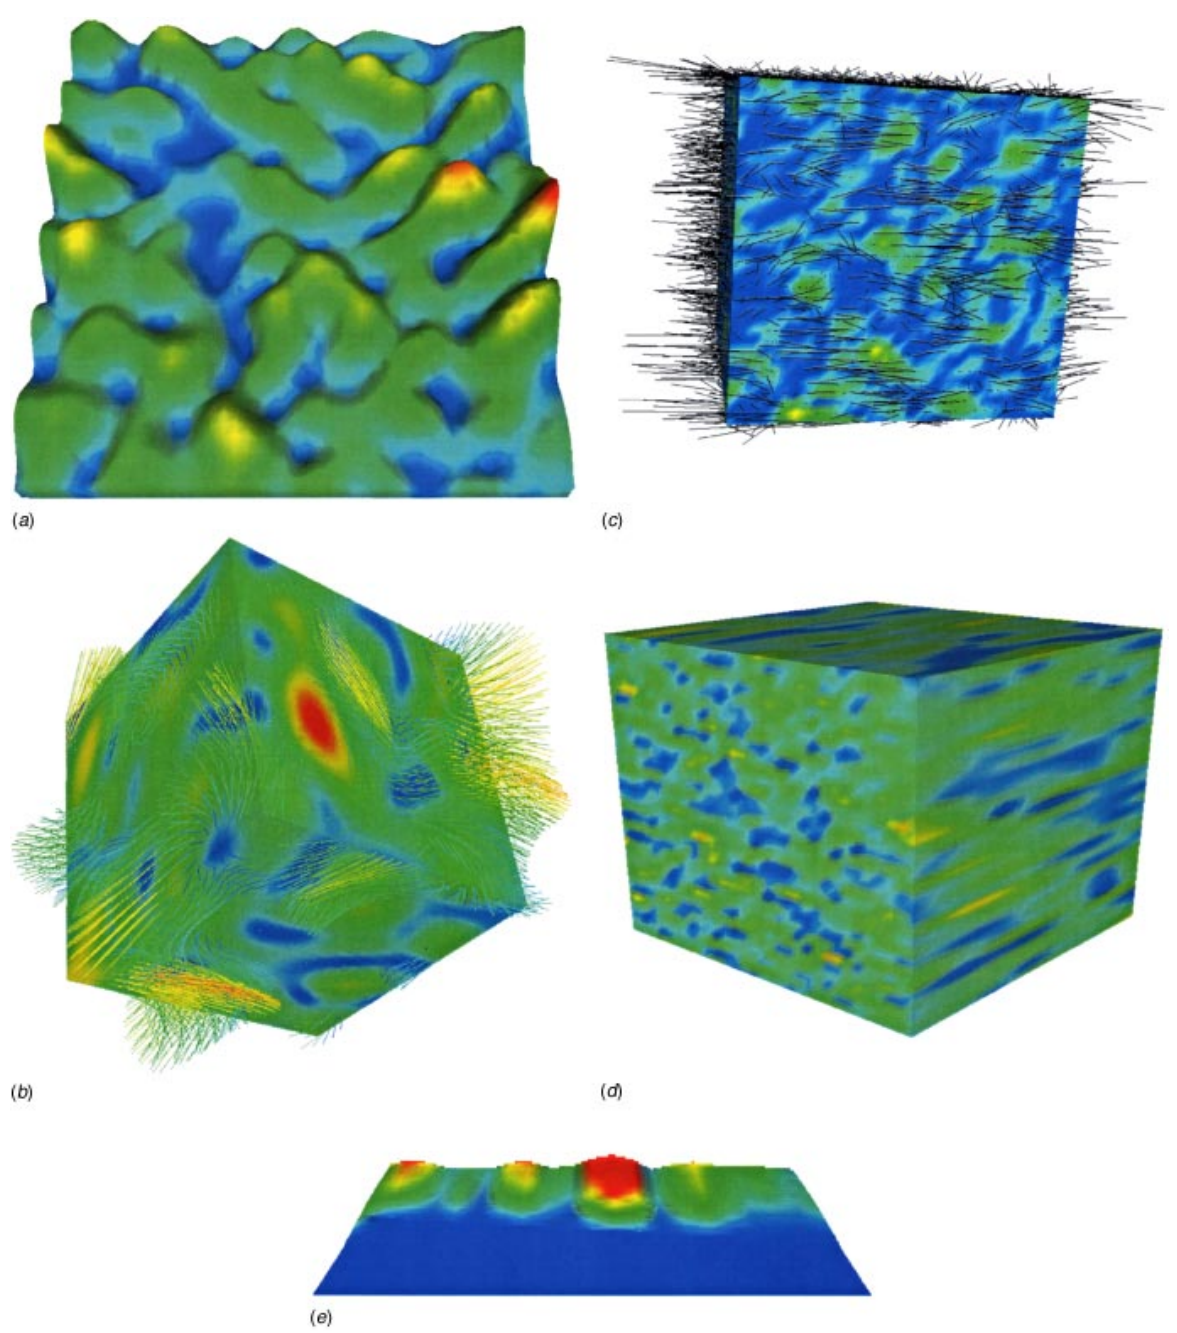
\includegraphics [width=0.6\linewidth] {smirnov_feilds}
  \caption{Сгенерированные авторами поля скоростей для a) изотропная завихрённость, b) изотропная скорость, c) анизотропная скорость d) анизотропный пространственный масштаб e) флуктуации на границе \cite{huang2010general}} 
  \label{img:smirnov_results}  
\end{figure}


\section{Метод Хуанга генерации синтетической турбулентности} \label{sect2_3}

Как упоминалось в секции \ref{sect2_2}, метод Смирнова задает базис для работы с генераций синтетической турбулентности. Как можно видеть, в методе присутствует достаточно большое число параметров. Эти параметры представляют собой, например, способ генерации случайных чисел, способ задания ряда Фурье, форма спектра, метод аппроксимации спектра, учет расстояний до стенок и тому подобное.
В методе используемым в статье~\cite{huang2010general} основное отличие заключается в используемом спектре. В методе Смирнова используется "Спектр Гаусса", который не так хорошо описывает реальный спектр при больших волновых числах. В работе Хуанга используется модифицированный спектр Вон-Кармана. Помимо этого используется специальный алгоритм аппроксимации спектра за счёт разложения его по меньшим частям. Однако вносимые в алгоритм правки, налагают дополнительные предположения, связанные с интегрируемостью флуктуации.

Ниже приведен график сравнения вида спектров используемых в работах Смирнова и Хуанга с близким к реальному спектром Вон-Кармана. Как можно видеть, в методе Смирнова спектр турбулентных флуктуаций не покрывает область больших волновых чисел. 

\begin{figure}[ht] 
  \center
  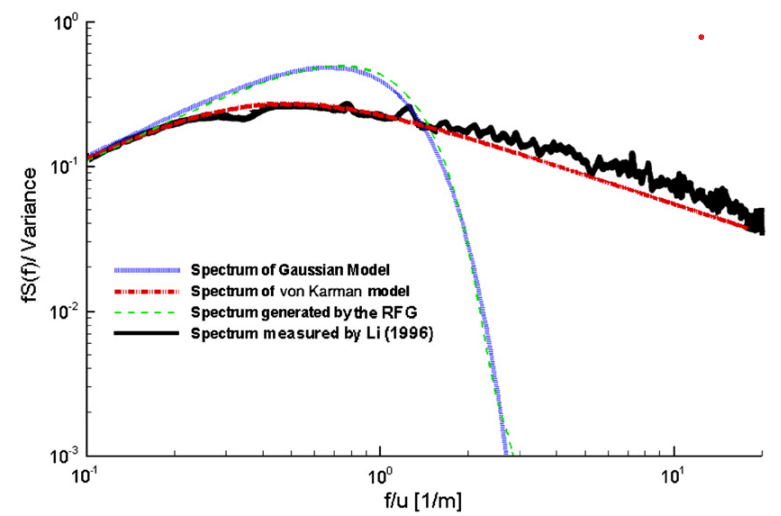
\includegraphics [] {huang_spect_rfg_smirnov_huang_li}
  \caption{Сравнение спектров для метода Смирнова со спектрами Вон-Кармана и спектром измеренным Ли\cite{huang2010general}} 
  \label{img:huang_spect_rfg_smirnov_huang_li}  
\end{figure}

На изображении \ref{img:huang_spect_rfg_smirnov_huang_li} показаны измерения для продольной компоненты флуктуации скорости потока ветра для процедуры генерации Смирнова с интенсивностью продольной турбулентности $I_u = 8 \%$ и интегральном масштабе турбулентности $L_u = 0.3 m$. Хорошо видно, что в области инерционного интервала для метода Смирнова наблюдается сильное затухание.

Как говорилось ранее, основная идея усовершенствования спектрального метода состоит в представлении целевого спектра в виде комбинации (суммы) небольших долей. Этот шаг можно назвать дополнительной дискретизации целевого спектра. За основу этих небольших долей берутся спектры, рассматриваемые нами ранее в работе Крайхнана \eqref{eq:spectral_equation2}. Авторы предлагают использовать для дискретизации спектры $E_1$ и $E_3$ для двумерного и трёхмерного случаев соответственно, в силу того, что они имеют ярко выраженный пик в значении $k = k_0$ и не влияют на другие "узлы" дискретизации. 

\begin{equation}
    \label{eq:spectral_equation14}
    E(k) = \sum_{m = k_0}^{k_{max}} E_m(k) = \sum_{m = k_0}^{k_{max}} E_m(k_m) \delta(k - k_m) = \sum_{m = k_0}^{k_{max}} \left( \frac{3}{2} v_m^2 \right) \delta(k - k_m)
\end{equation}

Теперь генерация, происходит для каждого слагаемого из суммы. Помимо этого, вводится явная зависимость между амплитудой получаемой скорости и значением энергии, соответствующее заданному волновому числу $k_m$. Стоит сразу отметить, что генерация поля скоростей для дискретизованного таким образом спектра, вносит дополнительную алгоритмическую сложность, в следствии необходимости дополнительных проходов генерации для каждого значения дискретизованного спектра. В этом случае флуктуация задается в виде:

\begin{equation}
    \label{eq:spectral_equation15}
    u_{m,i} = \sum_{n = 1}^{N} \left[ p_{i}^{m,n} \cos{(k_j^{m,n} \cdot x_j + \omega_n \cdot t)} 
        + q_{i}^{m,n} \cos{(k_j^{m,n} \cdot x_j + \omega_n \cdot t)}\right] 
\end{equation}
\noindent
здесь $k_i^{m,n}$ — изотропно распределенный вектор по сфере радиуса $k_m$, $\omega_{m, n} \in N(0, \omega_{m,n})$. Связывание амплитуд мод Фурье со значением спектра осуществляется по прямому определению значения $v_0$ — как среднеквадратичного отклонения скорости в любом направлении. Авторы выбирают следующее определение для нахождения связи:

\begin{equation}
    \label{eq:spectral_equation15_2}
    \sigma^2_{m,i} = \frac{1}{T} \int_{0}^{T} u_{m,i}^2 dt = \frac{2}{3} E_m(k_m) = \frac{2}{3} E(k_m) 
\end{equation}

В итоге получаем соотношение:

\begin{equation}
    \label{eq:spectral_equation15_3}
    \frac{1}{2} \sum_{n=1}^N \left[ p_i^{m,n} \right]^2 + \frac{1}{2} \sum_{n=1}^N \left[ q_i^{m,n} \right]^2 = \frac{2}{3} E(k_m) 
\end{equation}

Убедиться в этом можно прямой подстановкой \eqref{eq:spectral_equation15_2} в \eqref{eq:spectral_equation15}

\begin{align}
    & \frac{1}{T} \int_{0}^{T} u_{m,i}^2 dt = \nonumber \\ 
    & = \frac{1}{T} \int_{0}^{T} \left\{ \sum_{n = 1}^{N} \left[ p_{i}^{m,n} \cos{(k_j^{m,n} \cdot x_j + \omega_n \cdot t)} + q_{i}^{m,n} \cos{(k_j^{m,n} \cdot x_j + \omega_n \cdot t)}\right]  \right\}^2 dt                                                                          \nonumber \\
    & = \frac{1}{T} \sum_{n = 1}^{N} \left[p_i^{m,n}\right]^2 \frac{T}{2} + \frac{1}{T} \sum_{n = 1}^{N} \left[p_i^{m,n}\right]^2 \frac{T}{2} = \frac{1}{2} \sum_{n=1}^N \left[ p_i^{m,n} \right]^2 + \frac{1}{2} \sum_{n=1}^N \left[ q_i^{m,n} \right]^2 = \frac{2}{3} E(k_m)
\end{align}

Из вывода данной связи между значением энергии и мод Фурье вытекает, ранее упомянутое, требование к интегрируемости. В конечном итоге имеем в векторном виде следующие выражение:

\begin{equation}
    \label{eq:spectral_equation16}
    \frac{1}{2} \sum_{n}^N |\vec{p^{m,n}}|^2 + \frac{1}{2} \sum_{n}^N |\vec{q^{m,n}}|^2 = 2 E(k_m)
\end{equation}
\noindent
здесь записана система уравнений, связывающая амплитуды мод Фурье со значениями спектра для различных волновых чисел. Решать, данную систему можно различными способами. Первый наиболее очевидный способ использовать алгоритмы решения СЛАУ, но авторы поступили другим путём. Вводится дополнительная случайная величина $a$, через которую выражаются данные амплитуды. Это позволяет существенно сэкономить на решении СЛАУ, за счёт введения простой зависимости, а именно:

\begin{align}
    \label{eq:spectral_equation16_2}
    \vec{|p^{m,n}|} & = \sqrt{a \frac{4 E(k_m)}{N}} \nonumber \\
    \vec{|q^{m,n}|} & = \sqrt{(1 - a) \frac{4 E(k_m)}{N}}
\end{align}

Легко убедиться в том что данное выражение удовлетворяет уравнению \eqref{eq:spectral_equation16}, используя прямую подстановку:

\begin{equation}
    \frac{1}{2} \sum_{n}^N \vec{|p^{m,n}|}^2 + \frac{1}{2} \sum_{n}^N \vec{|q^{m,n}|}^2 = \frac{1}{2} \frac{4 E(k_m)}{N} \left[ 
    \sum_n^N a + \sum_n^N (1 - a) \right] = 2 E(k_m)
\end{equation}

Таким образом амплитуды мод Фурье, выражаются в виде:

\begin{equation}
    \label{eq:spectral_equation17_1}
    |\vec{p^{m,n}}| = \frac{\zeta \times \vec{k^{m,n}}}{|\zeta \times \vec{k^{m,n}}|} \sqrt{a \frac{4 E(k_m)}{N}}
\end{equation}
\begin{equation}
    \label{eq:spectral_equation17_2}
    |\vec{q^{m,n}}| = \frac{\zeta \times \vec{k^{m,n}}}{|\zeta \times \vec{k^{m,n}}|} \sqrt{(1 - a) \frac{4 E(k_m)}{N}}
\end{equation}

Авторы отмечают, что подход также требует корректировки значения пространственного масштаба турбулентности. Так как на самом деле оператор пространственной корреляции имеет зависимость от данного параметра:

\begin{equation}
    \label{eq:spectral_equation17}
    R(\vec x, \vec x') = \int_0^T \vec{u}(\vec x, t) \cdot \vec{u}(\vec x', t) dt \\
    = \sum_{m=k_0}^{k_{max}} \left\{ \frac{2 T E(k_m)}{N} \sum_{n=1}^N \cos{\left( \Tilde{\vec k}^{m,n} 
    \frac{\vec x - \vec x'}{L_s} \right)} \right\}
\end{equation}

Авторы предлагают, также, несколько иной подход к генерации анизотропной турбулентности, за счёт того, что имеется возможность разделить спектр на составляющие не только пространственно по-волновому вектора, но также и по компонентно. Разделим \eqref{eq:spectral_equation16} по компонентно в следующем виде:

\begin{equation}
    \label{eq:spectral_equation18}
    \frac{1}{2} \sum_{n}^N |\vec{p^{m,n}}|^2 + \frac{1}{2} \sum_{n}^N |\vec{q^{m,n}}|^2 = \frac{4}{3 N} E(k_m) = \frac{4}{N} E_i(k_m) 
\end{equation}

Как и до этого, введение случайного параметра по типу $a$, можно найти аналитическое выражение для задания амплитуд мод Фурье.

\begin{equation}
    \label{eq:spectral_equation18_1}
    p^{m,n}_i = \text{sign}(r_i^{m,n}) \sqrt{\frac{4}{N} E_i(k_m) \frac{(r_i^{m,n})^2}{1 + (r_i^{m,n})^2}}
\end{equation}
\begin{equation}
    \label{eq:spectral_equation18_2}
    q^{m,n}_i = \text{sign}(r_i^{m,n}) \sqrt{\frac{4}{N} E_i(k_m) \frac{1}{1 + (r_i^{m,n})^2}}
\end{equation}

Эта же процедура может использоваться и для генерации однородного поля скоростей путем задания одинакового спектра по всем пространственным направлениям. Стоит отметить, что с использованием матричных преобразований в методе Смирнова необходимо было, чтобы коэффициенты плавно менялись в пространстве для пренебрежения членами с их пространственными производными для удовлетворения уравнению неразрывности для случая генерации неоднородной и анизотропной турбулентности. В данном же случае, никаких подобных допущений не требуется, в результате чего уравнение неразрывности выполняется в точности.  

На валидации, авторам алгоритма удалось получить достаточно хорошее совпадение с целевым спектром. На рисунке ниже приведены результаты полученные авторами для трёх компонент флуктуаций скорости в сравнении со спектром Вон-Кармана. Параметры генерации те же, что использовались для сравнения для случая \ref{img:huang_spect_rfg_smirnov_huang_li}.

\begin{figure}[ht] 
  \center
  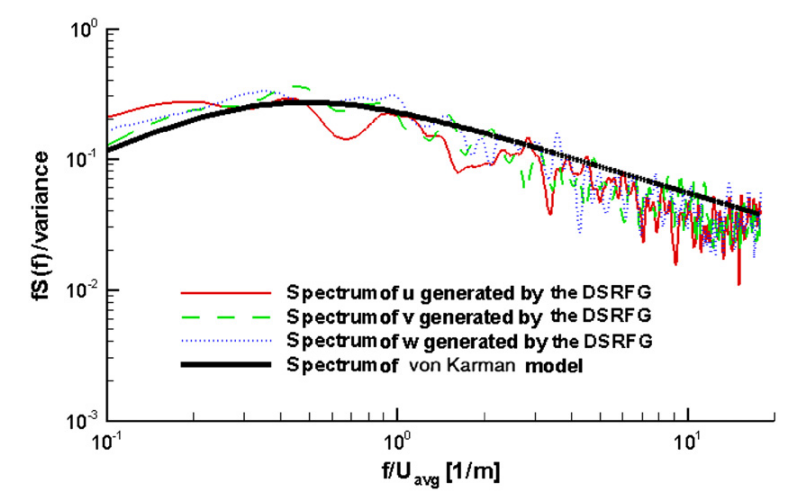
\includegraphics [] {huang_spect__huang_uvw}
  \caption{Сравнение результирующих спектров для сгенерированных компонент флуктуаций $u, v, w$ со спектром Вон-Кармана\cite{huang2010general}} 
  \label{img:huang_spect__huang_uvw}  
\end{figure}

\section{Метод Шура генерации синтетической турбулентности} \label{sect2_4}

Как упоминалось ранее, возможностей для изменения и корректировки метода открыто множество параметров. Один из них, внесение правок в сам алгоритм. Так в работе \cite{shur2014synthetic} вместо предложенным Смирновым ортогональных преобразований, используется разложение Холецкого для тензора напряжений Рейнольдса. Суть разложения Холецкого состоит в том, чтобы представить матрицу в виде произведения нижне треугольных матриц: $\hat{R} = \hat{A}^T \cdot \hat{A}$. Для прикладного случая - разложения тензора напряжений Рейнольдса, матрица $\hat{A}$ имеет вид:

\begin{equation}
    \label{eq:spectral_equation18_3}
     \hat{A} = a_{ij} = \begin{pmatrix}
                            \sqrt{R_{11}} & 0 & 0 \\
                            R_{21} / a_{11} & \sqrt{R_{22} - a_{21}^2} & 0 \\
                            R_{31} / a_{11} & \frac{R_{32} - a_{21} \cdot a_{31}}{a_22} & \sqrt{R_{33} - a_{31}^2 - a_{32}^2}
                        \end{pmatrix}
\end{equation}

Искомые флуктуации имеют вид:
\begin{equation}
    \label{eq:spectral_equation19}
    u_i(\vec r, t) = a_{ij} v_j(\vec r, t)
\end{equation}
\noindent
, где $v_j$ - компоненты генерируемы по принципу \eqref{eq:spectral_equation1}, но также налагая требование $<v_i v_j> = \delta_{ij}$. В общем случае, разложение $\hat{R} = \hat{A}^T \cdot \hat{A}$ не является однозадачным, например можно также использовать разложение на собственные числа и значения $\hat{R} = \hat{A}^T \cdot \hat{C} \cdot \hat{A} = \hat{A}^T \cdot \hat{C}^{\frac{1}{2}} \cdot \hat{C}^{\frac{1}{2}} \cdot \hat{A} = \hat{B}^T \cdot \hat{B}$, но для данного случая, необходимо чтобы собственные значениям были больше 0, или в более общем смысле, изначальная матрица положительно определена. Основная проблема в том что, в общем случае, матрица корреляций не отрицательно определена, и вполне могут быть встречены отрицательные собственные числа. 

Докажем то, что приводимое разложение действительно задает корреляцию наперед, пусть целевая матрица корреляций $R$, и случайная величина $\zeta \in N(0, 1)$. Результирующая случайная величина $\xi = \hat{A} \cdot \zeta$. 

\begin{equation}
    \label{eq:spectral_equation19_1}
    \mathbb{E} \left(\xi \xi^T\right) = \mathbb{E} \left((\hat{A} \zeta)(\hat{A} \zeta)^T \right) = \mathbb{E} \left(\hat{A} \zeta \zeta^T \hat{A}^T\right) = \hat{A} \mathbb{E} \left(\zeta \zeta^T \right) \hat{A}^T = \hat{A} \hat{A}^T = R
\end{equation}

Помимо использования другого метода получения анизотропной турбулентности, авторы также используют несколько изменённое определение для генерации флуктуации. 
\begin{equation}
    \label{eq:spectral_equation20}
    \vec{v}(\vec r, t) = 2 \sqrt{\dfrac{3}{2}} \sum_{n=1}^N \sqrt{q_n} \left[ \sigma^n \cos{(k^n \vec{d}^n \cdot 
    \vec r + \phi^n)} \right]
\end{equation}

здесь $N$ - число мод Фурье, $q^n$ - нормированная амплитуда моды фурье, $k^n$ - амплитуда волнового вектора, $d^n$ - случайно распределённый на единичной сфере вектор, $k^n = k^n \vec d^n$ ($\vec \sigma^n \cdot \vec d^n$). 

Принцип остается тот же, за исключением того, что зависимость от времени явно исключается из алгоритма. Таким образом авторы определяют все случайные величины всего один раз, так они не включают зависимость от времени, а также существенно упрощают алгоритм. При исключении явного рассмотрения времени из формул, необходимо каким-либо образом учесть нестационарность турбулентности. Чтобы учесть временную зависимость, авторы используют волновую конвекцию, вводится учёт волновой конвекции через компоненты псевдовектора положения $r'$.

\begin{equation}
    \label{eq:spectral_equation21}
    \vec r' = \left\{ \frac{2 \pi}{k^n \max{(l_e(\vec r)}} (x - U_0 t), y', z'\right\}
\end{equation}

здесь $U_0$ -макромашстабная величина скорости, $l_e$ -локальный пространственный масштаб вихрей.

Авторы также используют свою связь между амплитудами дискретизованного спектра и амплитудами мод Фурье.

\begin{equation}
    \label{eq:spectral_equation21_2}
    q^n = \frac{E(k_n) \Delta k^n}{\sum_{n=1}^N E(k_n) \Delta k^n}
\end{equation}

Это выражение удовлетворяют требованию нормированность амплитуд мод Фурье, а также в сравнении с \ref{sect2_3} имеет более простую форму, без введения дополнительных случайных параметров.

Как отмечалось ранее, в работе также используется спектр Вон-Кармана.

\begin{equation}
    \label{eq:spectral_equation22}
    E(k) = \frac{(\frac{k}{k_e})^4}{(1 + 2.4 \frac{k}{k_e})^2) ^ {\frac{17}{6}}} f_{\eta} f_{cut} 
\end{equation}

\begin{equation}
    \label{eq:spectral_equation23}
    f_{\eta} = \exp{(-(\frac{12 k}{k_\eta})^2)} 
\end{equation}

\begin{equation}
    \label{eq:spectral_equation23_1}
    f_{cut} = \exp{\left(-\left[ \frac{4 \max{(k - 0.9 k_{cut}), 0}}{k_{cut}} \right]^3\right)},\\
    k_{cut} = \dfrac{2 \pi}{l_{cut}} 
\end{equation}
\noindent
здесь $k_e = \frac{2 \pi}{l_e}$ - волновое число отвечающее за наиболее энергосодержащую моду. За счёт введения зависимости от локальных масштабов требуется высокая точность его определения для получения физической турбулентности на более маленьких длинах её развития. Авторы предполагают, что определяется как: $l_e = \min{2 d_w, C_l l_t}$, $d_w$ - расстояние от точки до ближайшей стенки, $C_l = 3,0$ - эмпирическая константа, $l_t$ - масштаб фоновой модели RANS ($l_t = \frac{k_t^\frac{1}{2}}{C_\mu \omega_t}$ для  $k-\omega$ модели). Для фильтрующих функций выбираются следующие параметры: $l_\mu = (\frac{\nu^3}{\epsilon})^\frac{1}{4}$. В демпфирующей функции: $l_{cut} = 2 \min{(\max{(h_y, hz, 0.3 h_{max})} + 0.1 d_w, h_{max})}$, $h_y,h_z$ - это локальные шаги сетки на интерфейсе RANS-LES, а $h_{max}=\max{(h_x,h_y,h_z)}$.

Так как распределение волновых чисел фиксируется, авторы используют геометрический ряд, для уменьшения количества волновых чисел: $k^n = k^{min}(1 + \alpha)^{n -1}, 0.01 \leq \alpha \leq 0.05$. Здесь $k^{min} = \beta k^{min}_e$ - минимальное волновое число в наборе, $\beta = 0.5$ - эмпирическая константа, $k^{min}_e$ - волновое число, соответствующее максимальному значению $l_e$ на интерфейсе, $l_e^{max} = \max{(l_e(\vec r))}$, $N$ - минимальное целое число для которого $k^N \geq k^{max} = 1.5 \max{k_{cut}(\vec r)}$. 

Суммируя алгоритм приведённый выше, используется фиксированный набор волновых чисел, также фиксированный по времени, и варьируется от значения соответствующего наибольшей длине волны в рассматриваемой задаче, до предела Нейквиста. Также спектра определяющий нормированные амплитуды в каждой точке имеет максимум при локально определённых волновых числах $k_e(\vec r) =\dfrac{2 \pi}{l_e(\vec r)}$, то-есть движется по фиксированному набору волновых чисел так, что моды с наибольшей длиной волны масштабируются малыми амплитудами вблизи стен, с наименьшей длиной волны масштабируются на малые амплитуды вдали от стен. Комбинация этих свойств STG обеспечивает образование сильно анизотропных (удлиненных) вихрей вблизи стенок и почти изотропных вихрей вдали от стенок.

Также все случайные величины входящие в \eqref{eq:spectral_equation20} определяются всего один раз, нивелируя высокочастотные флуктуации способствующее затуханию или ламинаризации ниже по потоку.
